% Lesson: the local coding fallback. OpenCode on the Mac, vLLM on AlfSPARK, over a tailnet tunnel.
% Compile with:  latexmk  (settings in .latexmkrc)

\documentclass[11pt,a4paper]{article}

\usepackage{fontspec}
\usepackage[margin=2.2cm]{geometry}
\usepackage{xcolor}
\usepackage[most]{tcolorbox}
\usepackage{listings}
\usepackage{twemojis}
\usepackage{lesson}
\usepackage{enumitem}
\usepackage{booktabs}
\usepackage{needspace}
\usepackage[colorlinks=true,linkcolor=blue,urlcolor=blue]{hyperref}
\usepackage{newunicodechar}
\newunicodechar{→}{\ensuremath{\rightarrow}}

% Recorded output is terminal output: Menlo keeps the look honest and carries the
% glyphs Latin Modern Mono lacks (✓ U+2713, the block art U+2580/84/88, ← and …).
\newfontface\termfont{Menlo}[Scale=MatchLowercase]
% ✓ must arrive through literate: listings defers unknown Unicode characters, which
% emitted every tick at the end of the previous line instead of its own.
\newcommand{\tick}{\hbox{\termfont ✓\char32}}
\lstdefinestyle{out}{
  basicstyle=\termfont\scriptsize\color{black!80}, columns=fullflexible, keepspaces=true,
  breaklines=true, breakatwhitespace=false, showstringspaces=false,
  moredelim=[is][\color{red!80!black}]{|!}{!|},
  moredelim=[is][\color{black!35}]{|~}{~|},
  literate={×}{{$\times$}}1 {→}{{$\rightarrow$}}1, escapechar=^
}
% The block-art banner stacks as a drawing: one block per text line, so its leading
% must close up. listings stacks each row as its own box: with lineskiplimit above the
% box height, TeX uses \lineskip for the row pitch, which is what actually lands.
% Menlo's box is 9.5pt tall against 6.3pt of block ink, so -3.2pt closes the gap to zero.
\lstdefinestyle{outtight}{
  basicstyle=\termfont\scriptsize\color{black!80}%
    \setlength{\baselineskip}{5pt}\setlength{\lineskiplimit}{20pt}\setlength{\lineskip}{-3.2pt}\selectfont,
  columns=fullflexible, keepspaces=true,
  breaklines=true, breakatwhitespace=false, showstringspaces=false,
  moredelim=[is][\color{red!80!black}]{|!}{!|},
  moredelim=[is][\color{black!35}]{|~}{~|},
  literate={×}{{$\times$}}1 {→}{{$\rightarrow$}}1, escapechar=^
}
\newtcblisting{cmdouttight}{listing engine=listings, listing only, enhanced, breakable,
  colback=white, colframe=black!25, boxrule=0.4pt, arc=1pt, left=4pt,
  title={Output}, fonttitle=\scriptsize, coltitle=black!70, colbacktitle=black!6,
  listing options={style=outtight}}

\setlength{\parindent}{0pt}
\setlength{\parskip}{0.6em}
\setlength{\emergencystretch}{3em}

\renewcommand{\panetitle}{A terminal on \name{AlfMAC5}}
\newcommand{\home}{\textasciitilde}  % the home folder, as the shell writes it

\newtcolorbox{result}[1]{enhanced, breakable, colback=green!22, colframe=green!50!black,
  colbacktitle=green!60, coltitle=black, title={\emo{check mark button}\ #1}, fonttitle=\bfseries, boxrule=1pt, arc=2pt}

\title{\emo{laptop}\ Local coding: OpenCode on the Mac, the model on \name{AlfSPARK}\\[0.3em]
  \large One harness, one model server, one source of instructions}
\author{Lesson for Alf, written by OpenCode}
\date{Sat 7 Nov 2026}

\begin{document}
\maketitle

\section*{Why this exists}

This project is both a backup and a private solution: it takes over when I cannot use \name{Claude Code} or \name{Codex}, and my code and conversations live only on machines I own, the Mac and \name{AlfSPARK}. \name{Claude Code} and \name{Codex} normally do their work through cloud services, and they stop when the Internet is down, when the service has an outage, or when my tokens run out. The \name{local-coding} project replaces them locally: the model runs on \name{AlfSPARK}, my \name{DGX Spark} (built on the NVIDIA \name{GB10 Grace Blackwell} chip: a 64-bit Arm CPU of twenty cores, ten fast \name{Cortex-X925} for the heavy work and ten power-saving \name{Cortex-A725} for the rest, 128 GB of unified memory, and a 4 TB self-encrypting solid-state drive~\cite{dgx}), and a coding harness on the Mac talks to it over the tailnet, so the work continues from inside my apartment. A \emph{harness} is the program that turns a model into an assistant: it hands the model tools to read files, edit them and run commands, and it carries out the model's instructions step by step~\cite{wwc}.

The design follows one rule: every assistant reads my instructions from the files I wrote for \name{Claude Code}, the global \name{CLAUDE.md} and the rule files. \name{Codex} already works this way: its \name{AGENTS.md} points at the same Claude files, and the OpenCode config was set up the same way (\S\ref{sec:rules}).

This lesson is the setup as it ran on Sat 7 Nov, when the model answered for the first time: four pieces, each with the command that starts it and the output that proves it is up.

\section{The picture}

Two machines: (a) \name{AlfSPARK}, the Spark that holds the model, and (b) \name{AlfMAC5}, the laptop I work on. Four pieces connect them, and the diagram repeats the labels.

\begin{enumerate}[leftmargin=2.2em,itemsep=2pt]
\item \textbf{the model server}: \name{vLLM} on (a) answers an OpenAI-compatible HTTP API on the Spark's own loopback address, so no machine, on the tailnet or anywhere else, can reach its port directly;
\item \textbf{the tunnel}: an \texttt{ssh -L} forward makes the Mac's \texttt{127.0.0.1:8000} the Spark's \texttt{127.0.0.1:8000}. SSH does travel over a network: the tailnet, the private one. The tunnel is the only door to the API, and \S\ref{sec:path} shows how it is built;
\item \textbf{the config}: one TOML file names the model, its server, and the two ports;
\item \textbf{the harness}: \name{OpenCode} on (b), running in the project home with my rules loaded.
\end{enumerate}

\begin{center}
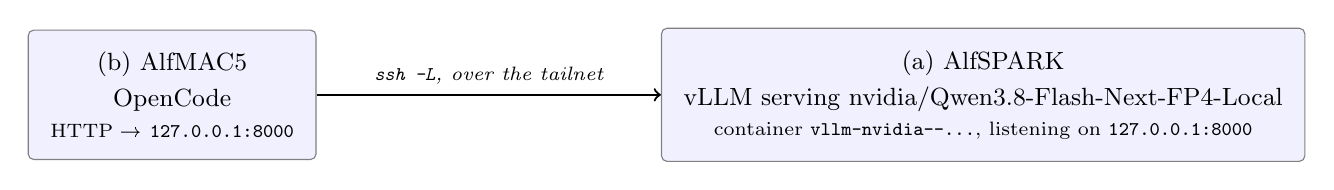
\begin{tikzpicture}[font=\small,
  mach/.style={draw=black!50, rounded corners=2pt, align=center, inner sep=8pt, fill=blue!6}]
  \node[mach] (mac) at (-5.8,0) {(b) \name{AlfMAC5}\\[2pt] \name{OpenCode}\\ \scriptsize HTTP → \texttt{127.0.0.1:8000}};
  \node[mach] (spark) at (4.5,0) {(a) \name{AlfSPARK}\\[2pt] \name{vLLM} serving \name{nvidia/Qwen3.8-Flash-Next-FP4-Local}\\ \scriptsize container \texttt{vllm-nvidia--\ldots}, listening on \texttt{127.0.0.1:8000}};
  \draw[thick,->] (mac.east) -- node[above,font=\scriptsize\itshape] {\texttt{ssh -L}, over the tailnet} (spark.west);
\end{tikzpicture}
\end{center}

\section{The operating cycle}

Day to day the setup is five verbs of one tool, \texttt{spark} (its source is \name{\home/.settings/Scripts/spark.py}, installed as \name{\home/.local/bin/spark}). The normal round trip begins with the machine off and works outward; each command is followed by its own output, as walked through on Sun 8 Nov. If \texttt{spark serve} finds the machine powered off, it first asks whether to turn it on, waits for the boot, and proceeds.

\begin{pane}
$ spark on --wait  # power on, block until SSH answers, print the boot time
\end{pane}
\begin{cmdout}
^\tick^ plug AlfSPARK: on
waiting for ssh alfspark…
^\tick^ alfspark up after 32 s
\end{cmdout}

\begin{pane}
$ spark serve      # serve the config default: vLLM with the Qwen model, open its tunnel, wait for its API
\end{pane}
\begin{cmdouttight}
^\tick^ vllm-nvidia--Qwen3.8-Flash-Next-FP4-Local: started
^\tick^ tunnel :8000 open
       █     █     █▄   ▄█
 ▄▄ ▄█ █     █     █ ▀▄▀ █  version 0.1.dev21830+g8244d1c44.d20261015
  █▄█▀ █     █     █     █  model   nvidia/Qwen3.8-Flash-Next-FP4-Local
   ▀▀  ▀▀▀▀▀ ▀▀▀▀▀ ▀     ▀
^\tick^ routing shards 21/21, 71.74 GB  2 min 53 s
^\tick^ routing shards 3/3, 4.14 GB  3 min 29 s
^\tick^ compiling decode CUDA graphs  3 min 51 s
^\tick^ compiling prefill CUDA graphs  3 min 55 s
^\tick^ API ready after 3 min 55 s
\end{cmdouttight}

The block-art banner is \name{vLLM}'s own opening lines, which \texttt{spark serve} shows as they land in the container's log. Asked twice, \texttt{spark serve} changes nothing: when the model already answers, it reports both facts as already true and waits nobody. The loading display reads the container's own log, one line kept on screen per completed phase, and the serve finishes when \texttt{http://127.0.0.1:8000/health} answers empty with HTTP 200.

\begin{pane}
$ spark s          # the five-line report (spark status)
\end{pane}
\begin{cmdout}
plug    AlfSPARK: on, 45.7 W -> alfspark running
tailnet alfspark: active; relay "nyc", tx 713174220 rx 223502956
service vllm (model nvidia/Qwen3.8-Flash-Next-FP4-Local): running 0 h 32 m
tunnel  AlfMAC5:8000 → alfspark:8000 open
api     AlfMAC5:8000: ready
\end{cmdout}

\begin{pane}
$ spark models     # the model store on the Spark
\end{pane}
\begin{cmdout}
  model                                           size  last access
  nvidia/Qwen3.8-Flash-Next-FP4-Local           102.3G  10 hours ago  ← served
\end{cmdout}

The status report keeps one fact per line. The model list is produced on the Spark by the \texttt{hf} command-line tool (Hugging Face's downloader), which reads the Hugging Face cache at \name{\home/.cache/\allowbreak huggingface/\allowbreak hub} from the path the config's \texttt{hf} key names.

\begin{pane}
$ spark unserve    # stop the vLLM service, close the tunnel it owns
\end{pane}
\begin{cmdout}
^\tick^ vllm-nvidia--Qwen3.8-Flash-Next-FP4-Local: stopped
^\tick^ tunnel :8000 closed
\end{cmdout}

\begin{pane}
$ spark off        # clean shutdown over ssh, then the plug
\end{pane}
\begin{cmdout}
shutting down alfspark (sudo asks for its password)
[sudo] password for atcold:
Connection to alfspark closed.
waiting for the draw to drop to standby…
^\tick^ alfspark shut down after 10 s
^\tick^ plug AlfSPARK: off
\end{cmdout}

\section{The model server, on \name{AlfSPARK}}

\begin{insight}{What vLLM is, and what else is out there}
\name{vLLM}~\cite{vllm} is an open-source inference server: it loads a model once, answers behind the OpenAI API, and keeps many requests flowing at once. It is one choice among several. \name{llama.cpp}~\cite{llama} is the C++ engine that runs quantized models on everything from a GPU to a phone; \name{Ollama}~\cite{oll} wraps it with model download and management, and \name{LM Studio}~\cite{lms} gives the same engine a desktop app. All of them can answer an OpenAI-compatible endpoint; \name{vLLM} was chosen because the community container built for the Spark runs on it~\cite{eug}.
\end{insight}

The server is \name{vLLM}, an OpenAI-compatible inference server, serving \name{nvidia/Qwen3.8-Flash-Next-FP4-Local}, NVIDIA's mixed-precision FP4 quantization of Flash-Next, about 102 GB of weights in the Hugging Face cache~\cite{nv}. The runtime is the community container \name{eugr/spark-vllm-b12x}, tag \name{nightly-20261015}: NVIDIA's own model card directs single-Spark users to community containers pending upstream support~\cite{nv}. The container was created once, from the published solo recipe's arguments (a GPU memory utilization budget of 0.8, covering the model and runtime allocations rather than only the key/value cache, a 262144-token context, multi-token prediction proposing up to 4 extra tokens per step, and 8 concurrent sequences), with the API bound to \texttt{127.0.0.1}.

 The running model is the NVIDIA checkpoint, revision \nolinkurl{b9ce18a6887e18c089fdea8509a33e63429a3300}. The runtime was launched by immutable image digest \nolinkurl{sha256:03a956544e9f9b4b7ba91690469fbe7848bdbef29a7d2e0f5788368467bb3595}. These identify the artifacts actually selected. The earlier community-modified weights remain a separate download; they are not the weights served here.

Three names keep to three facts. The \emph{service} is the \name{vLLM} server; the \emph{model} is \name{nvidia/Qwen3.8-Flash-Next-FP4-Local}; the container name is derived from the pair, the slash written \texttt{--}, giving \name{vllm-nvidia--Qwen3.8-Flash-Next-FP4-Local}. The naming is not cosmetic: it makes each container's identity say which server runs which model, so a second model, or a second server for the same model, is one more row of the config rather than a new idea. And whether a container really serves the id its name claims is checkable, not folklore: \texttt{docker inspect} on its launch command (\texttt{Config.Cmd}) names the model id the server was started with.

The whole machine-side picture lives in one TOML file, \name{\home/.config/spark/config.toml}; the commands take the default from it, so typing the long name is rare:

\begin{lstlisting}[style=out]
model = "nvidia/Qwen3.8-Flash-Next-FP4-Local"
hf = "~/voice-lab/hf/.venv/bin/hf"

[models]
# model = [server, local, remote]: the Mac listens on local, the
# Spark serves on remote; the container name is derived from the pair
"nvidia/Qwen3.8-Flash-Next-FP4-Local" = ["vllm", 8000, 8000]
\end{lstlisting}

The container was created once, without \texttt{--rm}, so it survives a stop and keeps its launch settings and internal caches; starting it and putting it away are one-word commands. Docker itself needs no \name{sudo} over SSH for this account: the one privileged moment was the image pull during installation.

\begin{tcolorbox}[enhanced, breakable, colback=white, opacityback=1, colframe=black!40, boxrule=0.5pt, arc=1pt, title={First start takes minutes}, colbacktitle=black!6, coltitle=black, fonttitle=\small\bfseries]
A cold start loads about 100 GB of weights and compiles the \name{B12X} kernels before the API answers, so \texttt{/health} fails for minutes while work is very much progressing. \texttt{spark serve} watches the container's own log through this window; the phase lines in The operating cycle are that watch, recorded. The endpoint itself is plain, and a browser can visit it once the tunnel is up:

\begin{pane}
$ curl -s http://127.0.0.1:8000/health   # empty body, exit 0, once served
\end{pane}

\end{tcolorbox}

\section{The path}
\label{sec:path}

On the Mac, one \texttt{ssh} puts a listener on the Mac's port 8000 and forwards every connection to the Spark's port 8000, over the tailnet. \texttt{-f} sends \texttt{ssh} to the background once connected, \texttt{-N} asks for no shell, only forwarding, \texttt{ExitOnForwardFailure=yes} makes \texttt{ssh} fail loudly instead of claiming success with the tunnel unmade (a port already taken by an old tunnel, say), and \texttt{ServerAliveInterval=30} sends a probe every 30 seconds so an idle tunnel is not dropped. In daily use \texttt{spark} opens this tunnel for the model it serves and closes it again on \texttt{unserve}, touching the listener only when it recognises its own \texttt{ssh} there; \texttt{spark status} then reports the tunnel and the API as two facts on two lines, since an open pipe and a ready server are different claims.

\begin{pane}
$ ssh -fN -o ExitOnForwardFailure=yes -o ServerAliveInterval=30 \
    -L 127.0.0.1:8000:127.0.0.1:8000 alfspark   # the tunnel, detached
$ ps aux | grep 'ssh -fN' | grep -v grep   # the tunnel is alive
\end{pane}
\begin{cmdout}
atcold 93184 ... ssh -fN -o ExitOnForwardFailure=yes -o ServerAliveInterval=30 |!-L 127.0.0.1:8000:127.0.0.1:8000 alfspark!|
\end{cmdout}

With the tunnel up, the Spark's API answers on the Mac's loopback:

\begin{pane}
$ curl -s http://127.0.0.1:8000/health && echo ' <- /health ok'   # through the tunnel
\end{pane}
\begin{cmdout}
 <- /health ok
\end{cmdout}

The first real request is the smallest completion: a chat turn that must reply with two words. The reply lands in \texttt{content}; the model's own thinking comes back separately in \texttt{reasoning}. The \texttt{system\_fingerprint} names the \name{vLLM} build, dated 20261015, consistent with the image tag. The fingerprint identifies a software build; the immutable digest above identifies the selected container image.

\begin{pane}
$ curl -s http://127.0.0.1:8000/v1/chat/completions \
    -H 'Content-Type: application/json' \
    -d '{"model": "nvidia/Qwen3.8-Flash-Next-FP4-Local",
         "messages": [{"role": "user", "content": "Reply with exactly: setup ok"}],
         "max_tokens": 64}'   # the smallest real request
\end{pane}
\begin{cmdout}
{"id":"chatcmpl-bd009f93eaef0691","model":"nvidia/Qwen3.8-Flash-Next-FP4-Local",
 "choices":[{"index":0,"message":{"role":"assistant",
   "content":"|!\n\nsetup ok!|",
   "reasoning":"|~We need to respond to user... Ensure no extra.~|"},
   "finish_reason":"stop", ...}],
 "system_fingerprint":"|!vllm-0.1.dev21830+g8244d1c44.d20261015!|", ...}
\end{cmdout}

\section{The harness, on \name{AlfMAC5}}

\begin{insight}{What OpenCode offers}
\name{OpenCode}~\cite{ocd} is an open-source coding agent: in a terminal (it also has desktop and editor faces) it runs the loop of read, edit, and shell against whichever model its config selects, with sessions that resume, per-command permission asks, and per-project configuration. It talks to any provider through a small adapter, which is exactly the seam the \texttt{spark} provider below sits in.
\end{insight}

\name{OpenCode} 1.19.5 is installed at \name{\home/\lk{.opencode}/bin/opencode}, not yet on \texttt{PATH}, so its full path is the command. Its config is one JSON file, \name{\home/Dropbox/Apps/\lk{opencode}/opencode.json}, linked at \name{\home/.config/\lk{opencode}/opencode.json}, the location OpenCode reads for every project~\cite{cfg}. The shared JSON is in Dropbox; the executable and configuration link have been installed on \name{AlfMAC5}. The key lines:

\begin{lstlisting}[style=out]
"model": "spark/nvidia/Qwen3.8-Flash-Next-FP4-Local",
"small_model": "spark/nvidia/Qwen3.8-Flash-Next-FP4-Local",
"enabled_providers": ["spark"],
"autoupdate": false,  "share": "disabled",
"provider": { "spark": {
    "npm": "@ai-sdk/openai-compatible",  "name": "AlfSPARK",
    "options": { "baseURL": "http://127.0.0.1:8000/v1",
                 "apiKey": "local",  "timeout": 600000 },
    "models": { "nvidia/Qwen3.8-Flash-Next-FP4-Local": {
        "reasoning": true,  "tool_call": true,
        "interleaved": { "field": "reasoning" },
        "limit": { "context": 262144,  "output": 32768 } } } }
\end{lstlisting}

The model is named twice on purpose: \texttt{model} answers the conversation, \texttt{small\_model} the background utility calls (titles, summaries). Both select the local inference endpoint. \texttt{enabled\_providers} narrows OpenCode to the one provider, \texttt{spark}, defined beside it as an OpenAI-compatible endpoint at the tunnel's address; the key is a placeholder because the server asks for none.  The \texttt{interleaved} field names \texttt{reasoning}, the key under which the \name{vLLM} server streams the model's thinking; a streaming request against the running container shows that key directly. The original setting, \texttt{reasoning\_content}, was a guess from a familiar \name{vLLM} convention, and a wrong name fails silently: the interface showed only a \texttt{Thought:} timer, never the thinking text. Whether that text renders at all is a separate switch, \texttt{display\_thinking}, which has no key by default and is bound to \texttt{<leader>d} in \name{tui.json}. With both in place, the reasoning sentences appear under the timer. \texttt{autoupdate} disables automatic application updates, and \texttt{share} disables session sharing; dependency downloads and other network activity still need an offline trial. The \texttt{edit} and \texttt{bash} permissions are set to ask, subject to approvals granted during a session.

\section{Reading my rules}
\label{sec:rules}

\begin{insight}{How OpenCode gets my instructions}
OpenCode's rules system loads an \texttt{AGENTS.md} found in the project and a global file, and the \texttt{instructions} field of the config names further files, read at startup and combined with them~\cite{rules}. It also reads \name{\home/.claude/CLAUDE.md} as a compatibility fallback when no global \texttt{AGENTS.md} exists. Our config lists the Claude originals by path, so the rules stay exactly where they are, one copy for both assistants:
\end{insight}

\begin{lstlisting}[style=out]
"instructions": [
  "~/.claude/CLAUDE.md",
  "~/.claude/rules/talking.md",  "~/.claude/rules/writing.md",
  "~/.claude/rules/git.md",      "~/.claude/rules/files.md",
  "~/.claude/rules/terminal.md", "~/.claude/rules/latex.md"
]
\end{lstlisting}

 Codex wrote this configuration during setup, using the same approach as its \name{AGENTS.md} adapter to point OpenCode's \texttt{instructions} list at the Claude originals.

The project's own context comes in at launch, not in the shared config. \texttt{OPENCODE\_CONFIG\_CONTENT} is an environment variable holding extra config JSON, merged over the files at startup; a relative \texttt{instructions} path resolves against the launch directory. Starting from the project home therefore adds that project's \texttt{note.md}, and a different project adds its own:

\begin{pane}
$ p lc   # cd ~/PARA/Projects/local-coding/, where note.md lives
$ OPENCODE_CONFIG_CONTENT='{"instructions": ["note.md"]}' ~/.opencode/bin/opencode .
\end{pane}

 The shared Bash settings now provide \texttt{oca}, beside \texttt{cca} and \texttt{cxa}. It expands to the same project-note configuration and OpenCode executable, with \texttt{--auto} added to accept permission requests automatically unless explicitly denied. Use \texttt{oca --continue} to resume the latest conversation in the current project.

The lesson you are reading is the proof of the whole chain: it was written by the Flash-Next model on \name{AlfSPARK}, asked through the tunnel, under the rule files it lists, with \name{note.md} open as the project's context.

\section{Starting a session}

A session from the Mac shell, start to finish. Everything between the plug and the API is \texttt{spark}'s: it drives \name{docker} over SSH (no \texttt{sudo}), opens the tunnel when it is missing, and waits for the API with the progress lines shown in The operating cycle. Those lines read \texttt{docker logs}, which \name{docker} writes to stderr rather than stdout, and the Spark's \name{docker} is too old for \texttt{--no-log-prefix}, so spark merges the streams and strips the timestamps itself; the phase names come from the container's own lines, such as \texttt{b12x routing checkpoint shards: 11/21 shards routed} and the CUDA-graph capture.

\begin{pane}
$ spark on --wait   # power on AlfSPARK and wait for SSH
$ spark serve       # start vLLM, open its tunnel, wait for the API
$ spark s           # confirm: service running, tunnel open, api ready
$ p lc              # enter this project home on the Mac
$ oca               # open OpenCode here, load note.md, and auto-accept requests
\end{pane}

For a different project, enter that project's PARA home instead of running \texttt{p lc}; the relative \texttt{note.md} then selects its own context. The current project is the directory shown when OpenCode opens.

Type \texttt{/exit} in OpenCode to return to the Mac shell. To leave a conversation and later resume it, start the same project with \texttt{--continue} appended to the OpenCode command. Stopping the harness leaves the model running; to stop inference and then the machine:

\begin{pane}
$ spark unserve   # stop vLLM, close the tunnel it owns
$ spark off       # optionally shut down AlfSPARK and switch off its plug
\end{pane}

\needspace{18\baselineskip}
\begin{thebibliography}{WWC}
  \bibitem[WWC]{wwc} \textit{How I work with Claude}, lesson in this repo: the harness idea and the local-coding goal. \url{../working-with-claude/}
  \bibitem[NV]{nv} NVIDIA, \textit{Qwen3.8-Flash-Next-FP4-Local}, model card. \url{https://huggingface.co/nvidia/Qwen3.8-Flash-Next-FP4-Local}
  \bibitem[Eug]{eug} \textit{spark-vllm-docker}, community containers for the DGX Spark. \url{https://github.com/eugr/spark-vllm-docker}
  \bibitem[OCc]{cfg} OpenCode, \textit{Config} documentation. \url{https://opencode.ai/docs/config/}
  \bibitem[OCr]{rules} OpenCode, \textit{Rules} documentation. \url{https://opencode.ai/docs/rules/}
  \bibitem[DGX]{dgx} NVIDIA, \textit{DGX Spark} product page and specifications. \url{https://www.nvidia.com/en-us/products/workstations/dgx-spark/}
  \bibitem[vLLM]{vllm} The \name{vLLM} project. \url{https://docs.vllm.ai/}
  \bibitem[LLa]{llama} \textit{llama.cpp}, C++ inference for large language models. \url{https://github.com/ggerganov/llama.cpp}
  \bibitem[Oll]{oll} \name{Ollama}, run large language models locally. \url{https://ollama.com/}
  \bibitem[LMS]{lms} \name{LM Studio}, desktop app for local models. \url{https://lmstudio.ai/}
  \bibitem[OCt]{ocd} OpenCode, \textit{Introduction} documentation. \url{https://opencode.ai/docs/}
\end{thebibliography}

\end{document}
